\documentclass[border=10pt]{standalone}
\usepackage{tikz}
\usetikzlibrary{shapes, positioning, arrows.meta, calc}

\begin{document}
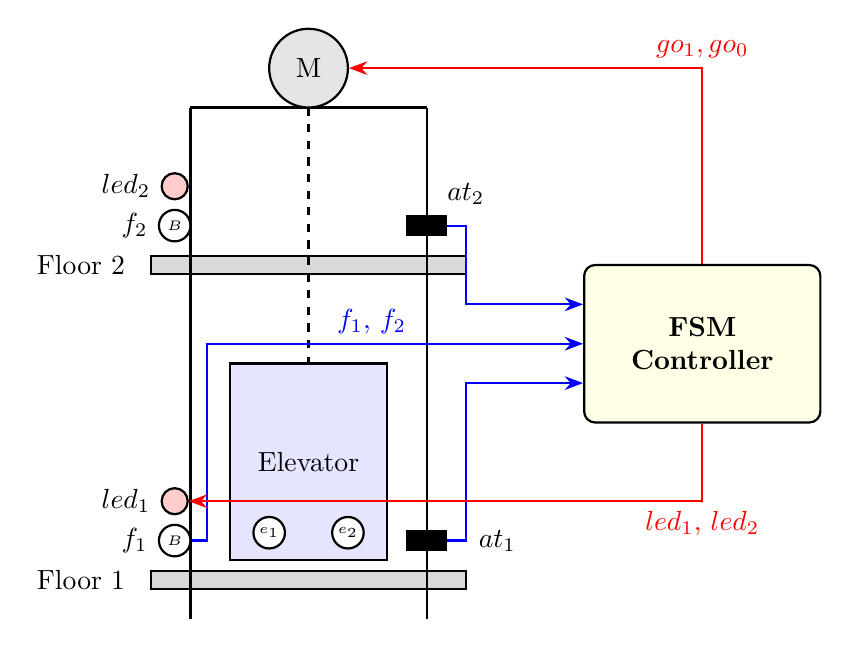
\begin{tikzpicture}[
    thick,
    >=Stealth,
    floor/.style={draw, minimum width=4cm, minimum height=0.2cm, fill=gray!30},
    button/.style={circle, draw, fill=white, inner sep=1pt, minimum size=0.4cm, font=\tiny},
    sensor/.style={rectangle, draw, fill=black, minimum width=0.5cm, minimum height=0.2cm},
    led/.style={circle, draw, fill=red!20, minimum size=0.3cm}
]

    % Building structure
    % Floor 1
    \node[floor] (f1_floor) at (0, 0) {};
    \node[left] at (-2.2, 0) {Floor 1};
    
    % Floor 2
    \node[floor] (f2_floor) at (0, 4) {};
    \node[left] at (-2.2, 4) {Floor 2};

    % Shaft walls
    \draw (-1.5, -0.5) -- (-1.5, 6);
    \draw (1.5, -0.5) -- (1.5, 6);
    \draw (-1.5, 6) -- (1.5, 6); % Roof

    % Elevator Car
    \node[draw, rectangle, minimum width=2cm, minimum height=2.5cm, fill=blue!10] (car) at (0, 1.5) {Elevator};
    
    % Internal Buttons
    \node[button] at (-0.5, 0.6) (e1) {$e_1$};
    \node[button] at (0.5, 0.6) (e2) {$e_2$};

    % Sensors (Limit Switches)
    \node[sensor] (at1) at (1.5, 0.5) {}; 
    \node[label=right:{$at_1$}] (at1_label) at (1.9, 0.5) {};
    \node[sensor, label=above right:{$at_2$}] (at2) at (1.5, 4.5) {};

    % Floor Buttons (External)
    \node[button, label=left:{$f_1$}] (f1) at (-1.7, 0.5) {$B$};
    \node[button, label=left:{$f_2$}] (f2) at (-1.7, 4.5) {$B$};
    
    % Floor LEDs
    \node[led, label=left:{$led_1$}] (l1) at (-1.7, 1.0) {};
    \node[led, label=left:{$led_2$}] (l2) at (-1.7, 5.0) {};

    % Motor
    \node[draw, circle, minimum size=1cm, fill=gray!20] (motor) at (0, 6.5) {M};
    \draw (motor.south) -- (0, 6); % Shaft connection
    % Cable
    \draw[dashed] (0, 6) -- (car.north);

    % Controller Box (Abstract)
    \node[draw, rectangle, rounded corners, minimum width=3cm, minimum height=2cm, align=center, fill=yellow!10] (ctrl) at (5, 3) {\textbf{FSM} \\ \textbf{Controller}};

    % Connections
    % Inputs to Controller
    \draw[->, blue] (at1) -- ++(0.5, 0) |- ($(ctrl.west)+(0, -0.5)$);
    \draw[->, blue] (at2) -- ++(0.5, 0) |- ($(ctrl.west)+(0, 0.5)$);
    \draw[->, blue] (f1.east) -- ++(0.2, 0) coordinate(f1_tap) -- (f1_tap |- ctrl.west) -- (ctrl.west) node[midway,above][xshift=-0.3cm] {$f_1$, $f_2$};
    % Grouping f2/f1 wire visually simplified
    
    % Outputs from Controller
    \draw[->, red] (ctrl.north) -- ++(0, 1) |- (motor.east) node[midway, above] {$go_1, go_0$};
    \draw[->, red] (ctrl.south) -- ++(0, -1) |- (l1.east) node[midway, below] {$led_1$, $led_2$};
    
\end{tikzpicture}
\end{document}
